
\includegraphics[height=1.25cm]{images/pictograms/FEM}

%%%%%%%%%%%%%%%%%%%%%%%%%%%%%%%%%%%%%%%%%%%%%%%%%%%%%%%%%%%%%%%%%%%%%%%%%%%%%%%%%%%%%%%%%



\lstinputlisting[language=bash,basicstyle=\small]{python_codes/fieldstone_02/keywords.ascii}

\begin{center}
Code at \url{https://github.com/cedrict/fieldstone/tree/master/python_codes/fieldstone_02}
\end{center}

\par\noindent\rule{\textwidth}{0.4pt}
%%%%%%%%%%%%%%%%%%%%%%%%%%%%%%%%%%%%%%%%%%%%%%%%%%%%%%%%%%%%%%%%%%%%%%%%%%%%%%%%%%%%%%%%%

This stone carries out the benchmark of Section~\ref{MMM-ss:stokes_sphere2D}
with $Q_1\times P_0$ elements using the penalty formulation.
The domain is a unit square and the fluid is characterised 
by $\rho=1$ and $\eta=1$ 
while the sphere is characterised 
by $\rho=1.01$ and $\eta=1000$.
The gravity vector is $\vec{g}=(0,-1)$. 

Boundary conditions are free slip on all sides ({\tt bc\_type=0}), 
no slip on all sides ({\tt bc\_type=1}) or free slip on the sides and bottom and open 
on top ({\tt bc\_type=2}).
Viscosity and density directly computed at the quadrature points.
The results are presented in Section~\ref{MMM-ss:stokes_sphere2D} and compared to 
those obtained with other codes.

Also, because of the inherent symmetry we can solve the system 
on only half the domain:
\begin{center}
\includegraphics[width=3cm]{python_codes/fieldstone_02/results/eta_1}
$\rightarrow$
\includegraphics[width=3cm]{python_codes/fieldstone_02/results/eta_2}
\end{center}


\begin{center}
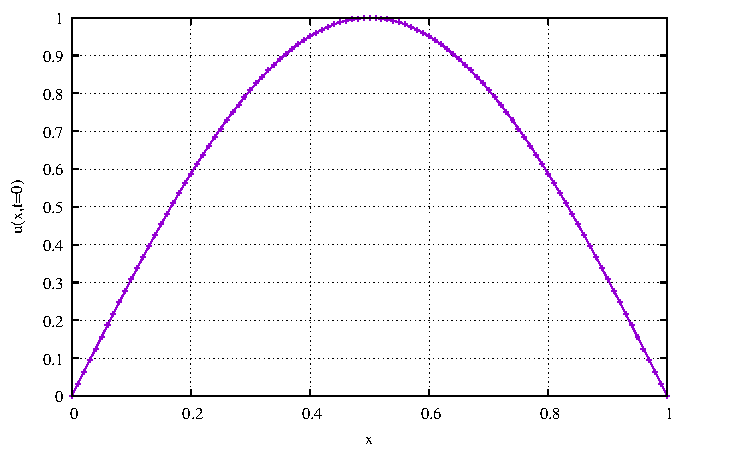
\includegraphics[width=3cm]{python_codes/fieldstone_02/results/u0}
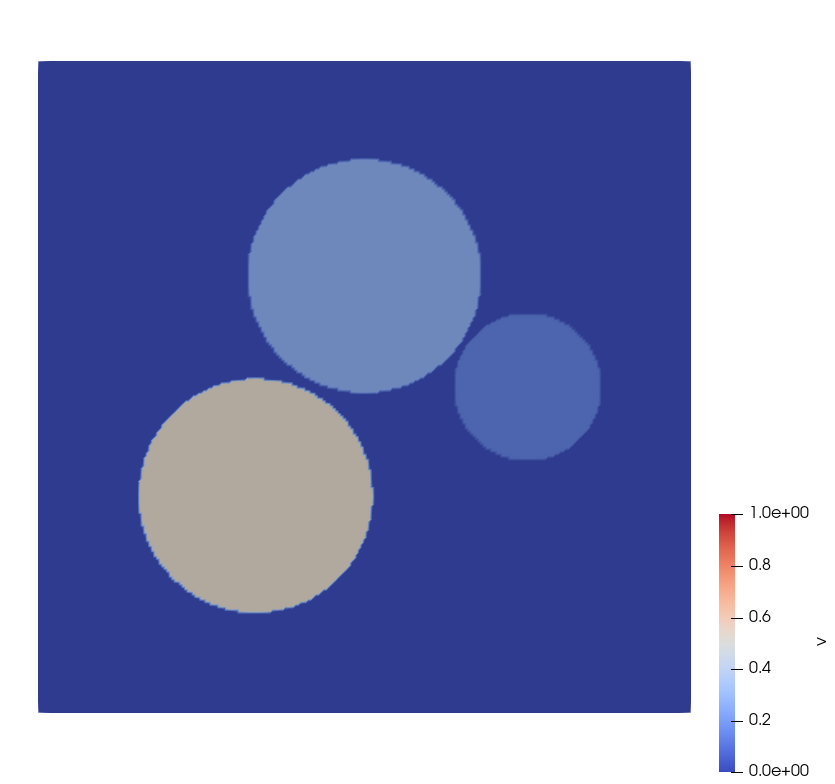
\includegraphics[width=3cm]{python_codes/fieldstone_02/results/v0}
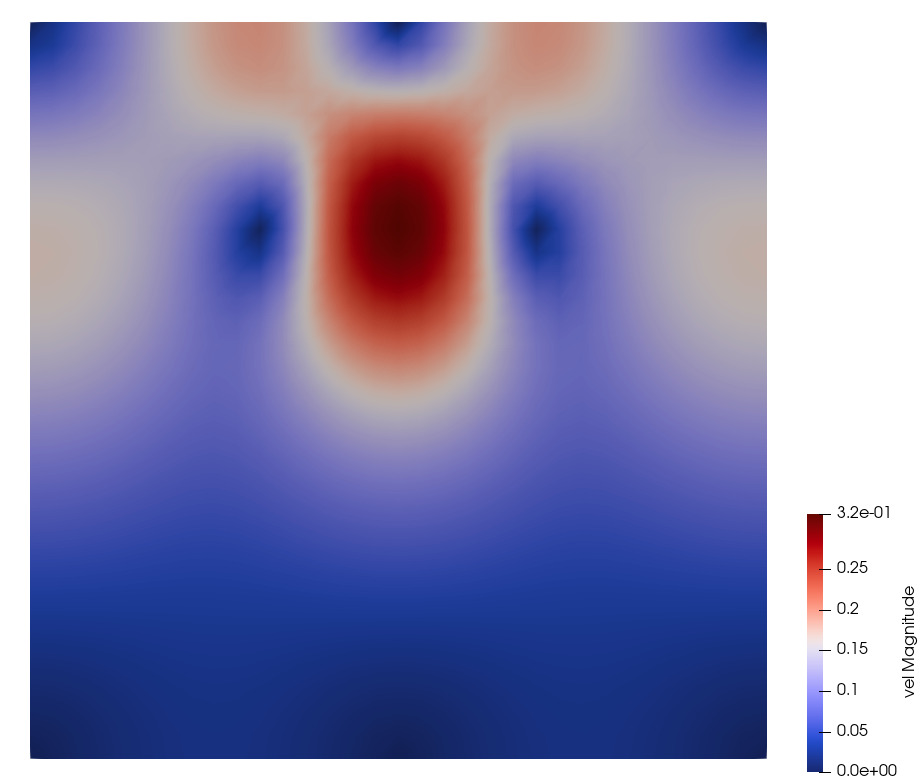
\includegraphics[width=3cm]{python_codes/fieldstone_02/results/vel0}
\includegraphics[width=3cm]{python_codes/fieldstone_02/results/sr0}
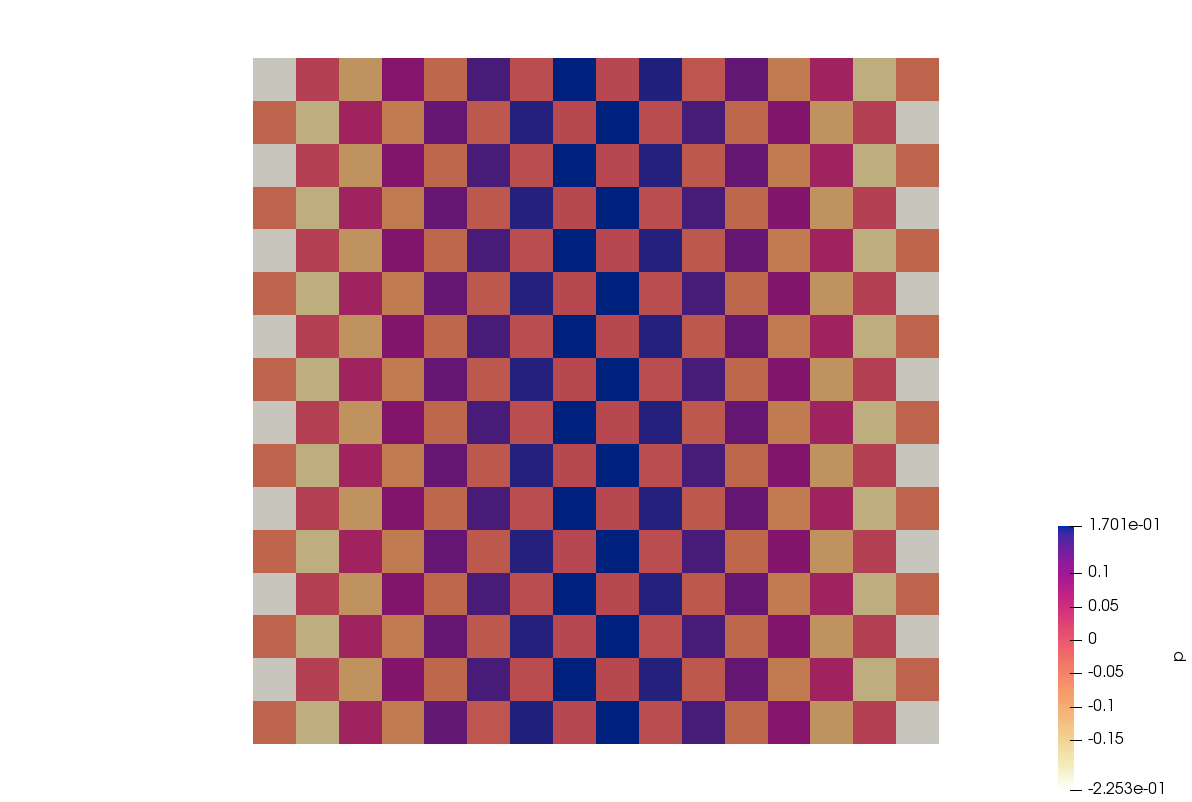
\includegraphics[width=3cm]{python_codes/fieldstone_02/results/p0}\\
\includegraphics[width=3cm]{python_codes/fieldstone_02/results/u1}
\includegraphics[width=3cm]{python_codes/fieldstone_02/results/v1}
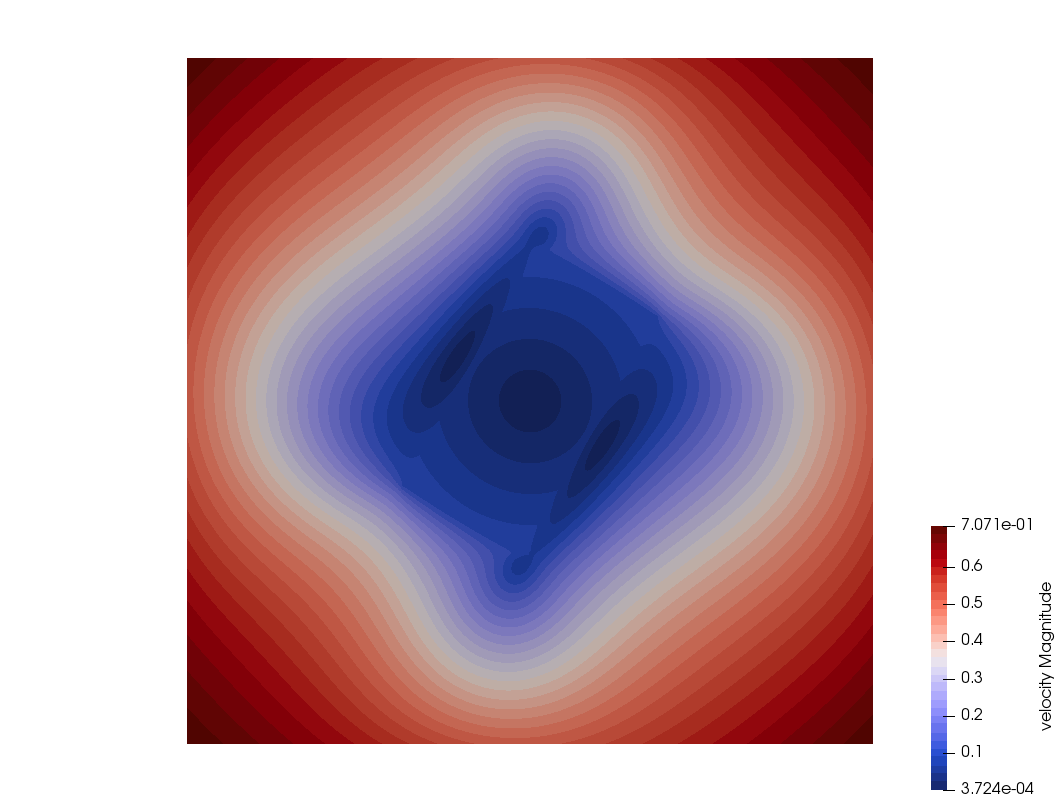
\includegraphics[width=3cm]{python_codes/fieldstone_02/results/vel1}
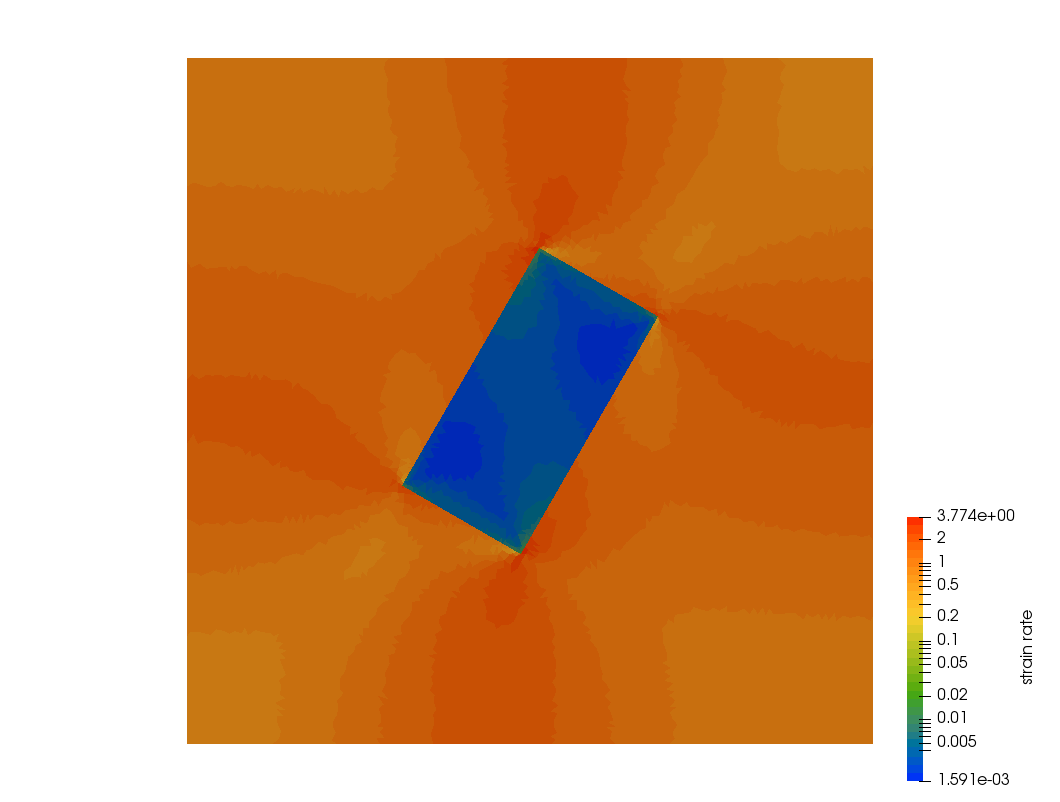
\includegraphics[width=3cm]{python_codes/fieldstone_02/results/sr1}
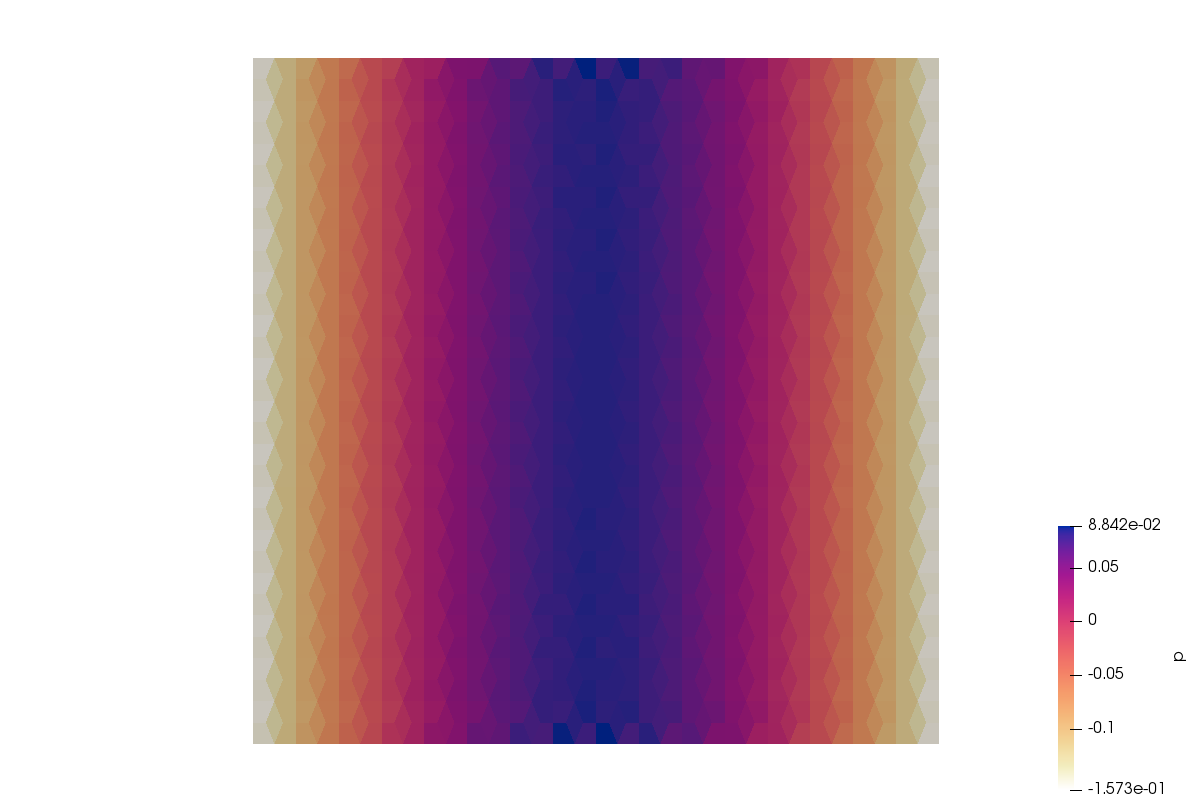
\includegraphics[width=3cm]{python_codes/fieldstone_02/results/p1}\\
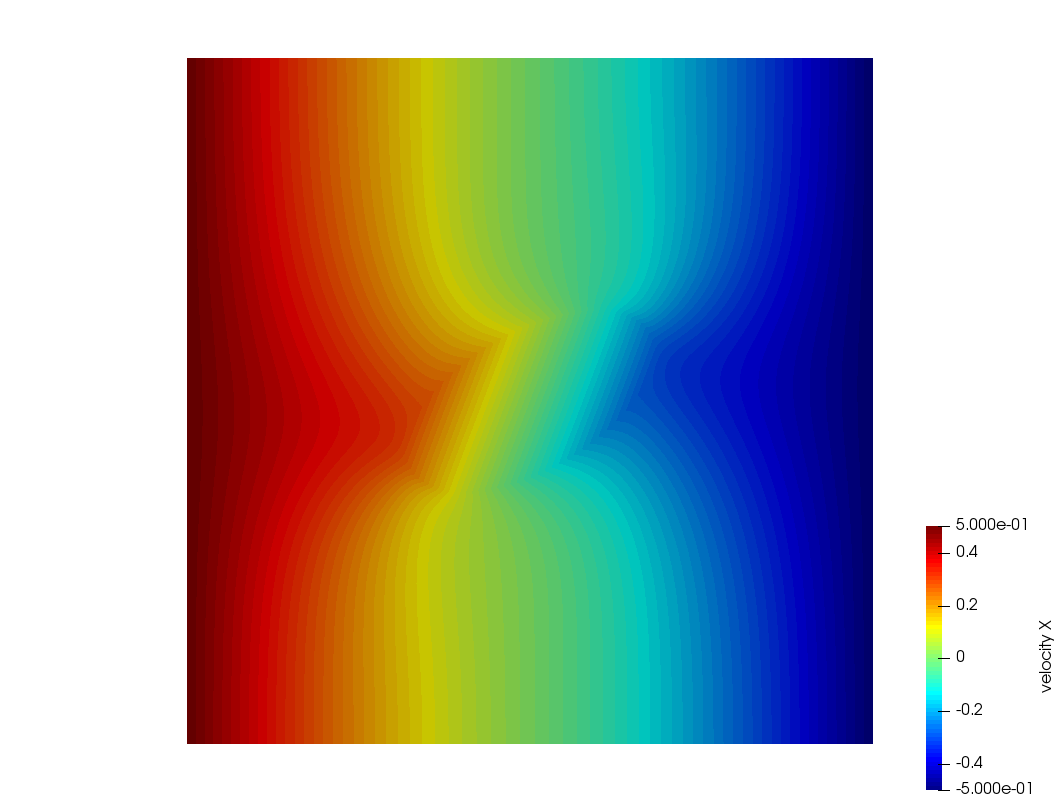
\includegraphics[width=3cm]{python_codes/fieldstone_02/results/u2}
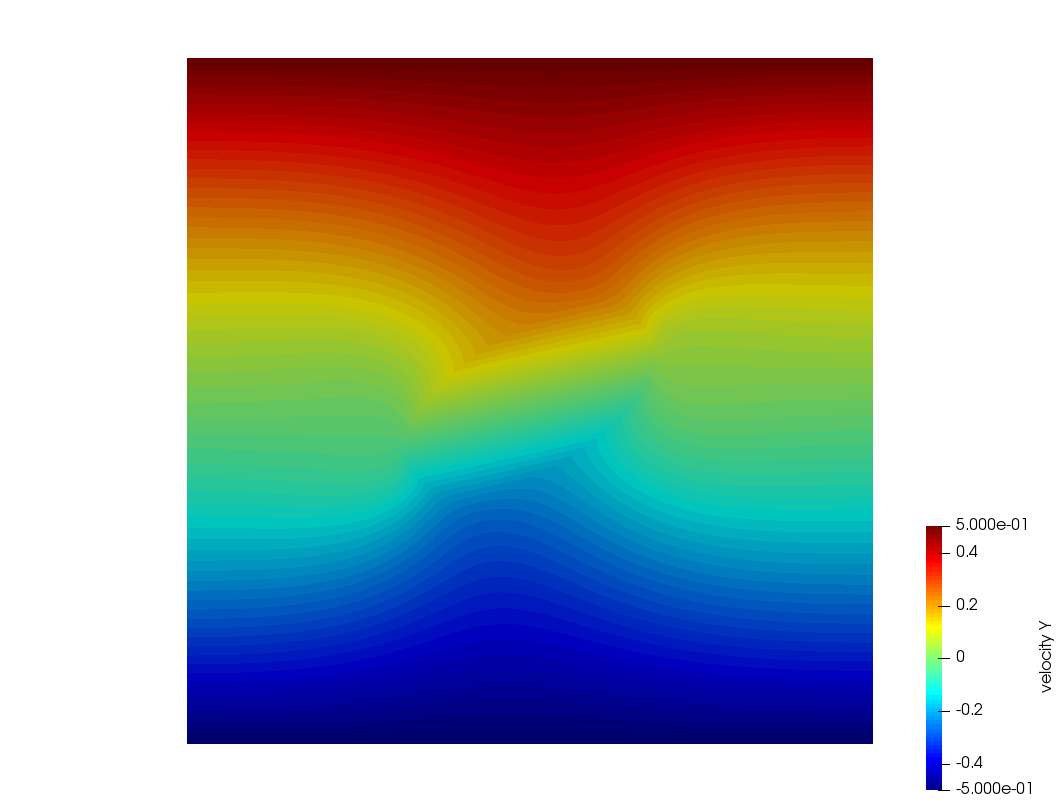
\includegraphics[width=3cm]{python_codes/fieldstone_02/results/v2}
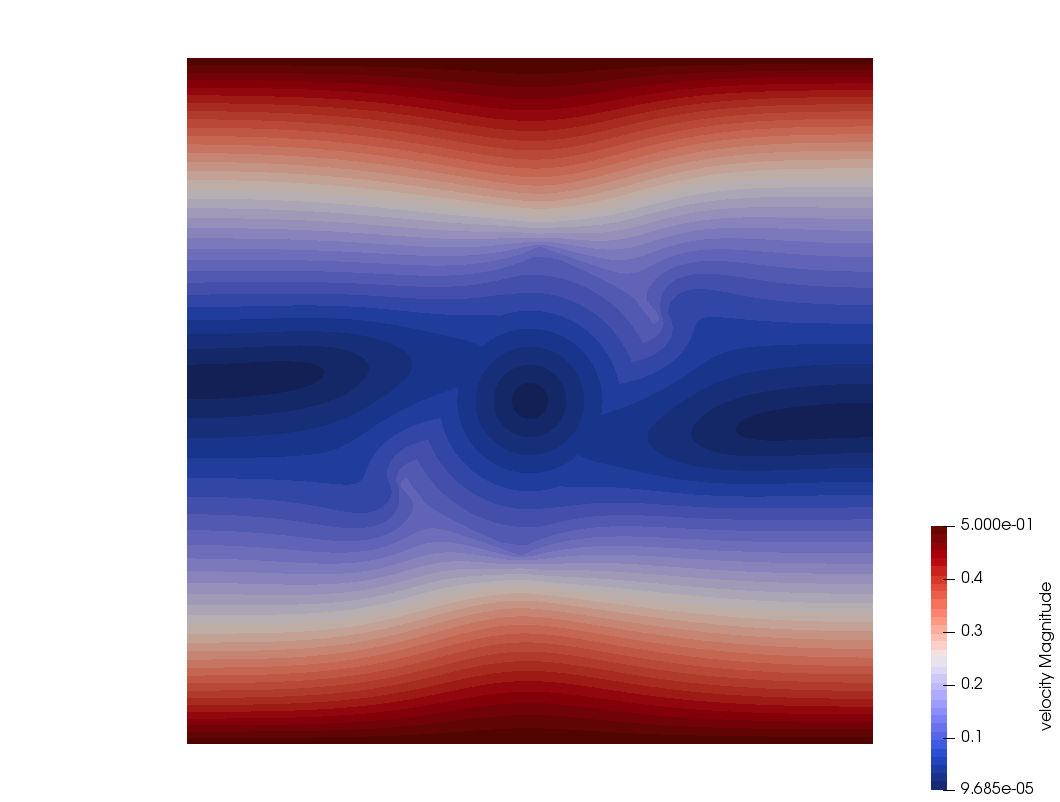
\includegraphics[width=3cm]{python_codes/fieldstone_02/results/vel2}
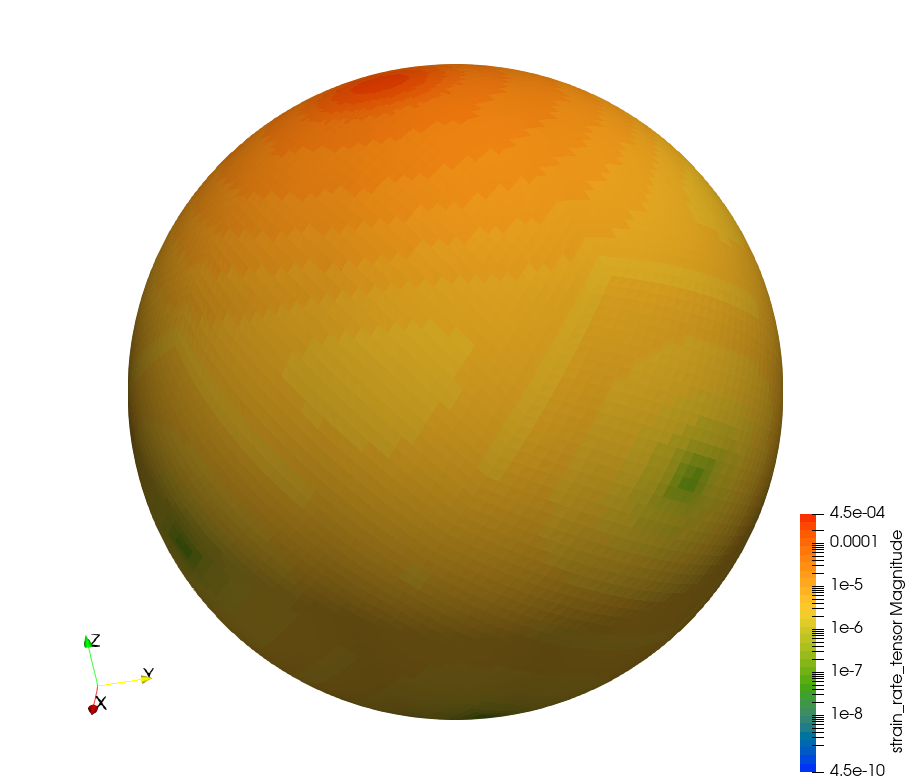
\includegraphics[width=3cm]{python_codes/fieldstone_02/results/sr2}
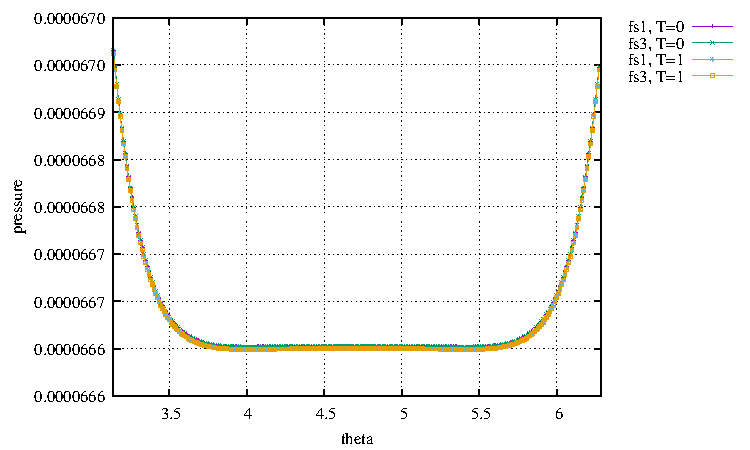
\includegraphics[width=3cm]{python_codes/fieldstone_02/results/p2}\\
{\captionfont Results on a $32\times 64$ grid. Top is free-slip, 
middle is no-slip, bottom is open top.}
\end{center}


